\documentclass[a4paper]{extarticle}
\usepackage[utf8]{inputenc}
\usepackage[a4paper, margin=1in]{geometry}

\usepackage{amssymb}
\usepackage{amsmath}
\usepackage{enumitem}
\usepackage{tcolorbox}
\usepackage{fancyhdr}
\usepackage{graphicx}
\usepackage{float}

\setlength{\parindent}{0em}
\setlength{\parskip}{0.4em}

\definecolor{theoremblue}{RGB}{1, 73, 124}
\definecolor{corollaryblue}{RGB}{70, 143, 175}
\definecolor{exampleblue}{RGB}{137, 194, 217}

\newtcolorbox{tbox}{colback=theoremblue!20,colframe=theoremblue,
boxrule=0pt,arc=0pt,boxsep=2pt,left=2pt,right=2pt,leftrule=2pt}

\newtcolorbox{cbox}{colback=corollaryblue!20,colframe=corollaryblue,
boxrule=0pt,arc=0pt,boxsep=2pt,left=2pt,right=2pt,leftrule=2pt}

\newtcolorbox{ebox}{colback=exampleblue!20,colframe=exampleblue,
boxrule=0pt,arc=0pt,boxsep=2pt,left=2pt,right=2pt,leftrule=2pt}

\title{FMFP - Lecture Notes Week 4}
\author{Ruben Schenk, ruben.schenk@inf.ethz.ch}
\date{\today}

\pagestyle{fancy}
\fancyhf{}
\rhead{ruben.schenk@inf.ethz.ch}
\rfoot{Page \thepage}
\lhead{FMFP - Lecture Notes Week 4}

\begin{document}

\maketitle
\newpage

\subsubsection{Partial Application}

Functions of multiple arguments can be \textbf{partially applied.} Consider the following example:

\begin{verbatim}
    multiply :: Int -> Int -> Int
    multiply a b = a * b

    ? :type multiply 7
    Int -> Int

    ? :type map
    (a -> b) -> [a] -> [b]

    ? map (multiply 7) [1, 2, 3, 4]
    [7, 14, 21, 28] :: [Int]
\end{verbatim}

It is important to note here that each function takes \textit{exactly one argument!} Consider\\ \verb|multiply :: Int -> Int -> Int| means \verb|multiply :: Int -> (Int -> Int)|. Therefore, the application \verb|multiply 2 3| means \verb|(multiply 2) 3|.

Furthermore, we might use \textbf{tuple arguments.} They may are equivalent to multiple-argument functions, however they do no not allow partial application!

\section{Higher-Order Programming and Types}

\subsection{Overview}

\subsubsection{Implement a Function with foldr}

\begin{figure}[H]
    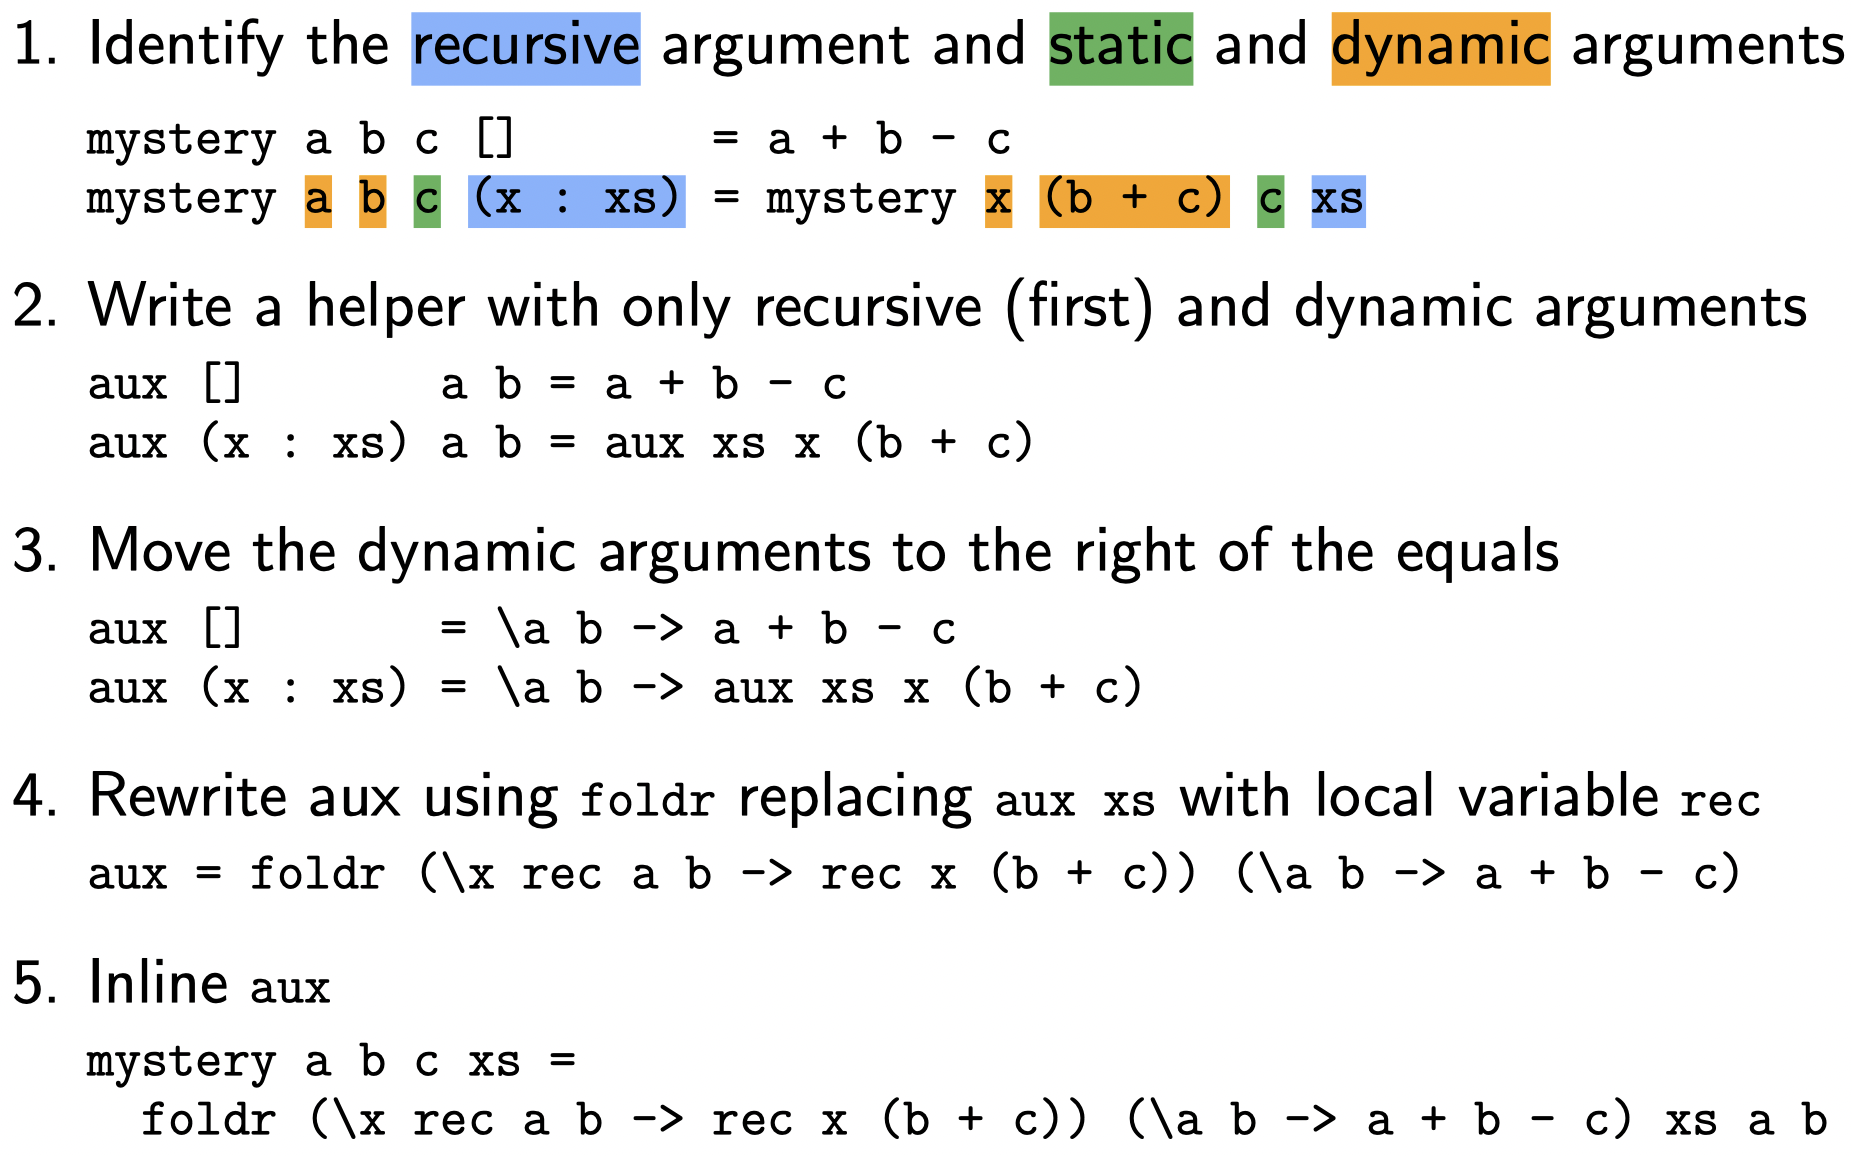
\includegraphics[width=13cm]{../images/FMFP_Fig4-1}
    \centering
\end{figure}

\subsection{Case Study: Operations on Vectors and Matrices}

\textbf{Vectors} and vector addition can be easily defined by:

\begin{verbatim}
    type Vector = [Int]

    vecAdd :: Vector -> Vector -> Vector
    vecAdd (x:xs) (y:ys) = (x + y) : vecAdd xs ys
    vecAdd _             = []
\end{verbatim}

We could also use \verb|zipWith|, which is a combination of \verb|map| and \verb|zip|. This would look as follows:

\begin{verbatim}
    vecAdd :: Vector -> Vector -> Vector
    vecAdd = zipWith (+)
\end{verbatim}

An \(n \times m\) \textbf{matrix} can be represented \textit{column-wise} using lists. We might write this like:

\begin{verbatim}
    type Matrix = [Vector]

    matAdd :: Matrix -> Matrix -> Matrix
    matAdd = zipWith vecAdd
\end{verbatim}

Some other matrix-related definitions:

\begin{verbatim}
    -- Constant vector of size n
    vconst :: Int -> Int -> Vector
    vconst 0 _ = []
    vconst n x = x : vconst (n - 1) x

    -- unit matrix of size n x n
    unit :: Int -> Matrix
    unit 0 = []
    unit n =
        (1 : vconst (n - 1) 0)
        : map (0:) (unit (n - 1))
\end{verbatim}

\textbf{Transposing} of a matrix can be implemented as follows:

\begin{verbatim}
    tr :: Matrix -> Matrix
    tr []       = []
    tr [v]      = map (\x -> [x]) v
    tr (v:vs)   = zipWith (:) v (tr vs)
\end{verbatim}

Another very important operation in linear algebra is the \textbf{dot product.} We propose different ways to implement it in Haskell:

\begin{verbatim}
    -- Version 1: Loop / accumulator
    skProd :: Vector -> Vector -> Int
    skProd xs ys = loop xs ys 0
        where
            loop []     []     0 = p
            loop (x:xs) (y:ys) p = loop xs ys (x * y + p)

    -- Version 2: Explicit recursion
    skProd :: Vector -> Vector -> Int
    skProd (x:xs) (y:ys) = x * y + skProd xy ys
    skProd _      _      = 0

    -- Version 3: Using library functions
    skProd :: Vector -> Vector -> Int
    skProd v w = sum (zipWith (*) v w)
\end{verbatim}

Finally, we can go to the most interesting problem: \textbf{matrix multiplication.} WE first start by multiplying an \(n \times m\) matrix \(A\) with vector \(b\) of size \(m\), which is equivalent to the scalar product of \(A\)'s rows (i.e. the columns of \verb|tr| \(A\)) with \(b\):

\begin{verbatim}
    vecMult :: Matrix -> Vector -> Vector
    vecMult a b = map ('skProd' b) (tr a)
\end{verbatim}

With this problem solved, matrix multiplication simply iterates \verb|vecMult| \(A\) over an \(m \times k\) matrix \(B\):

\begin{verbatim}
    matMult :: Matrix -> Matrix -> matrix
    matMult a b = map (vecMult a) b
\end{verbatim}

\end{document}